% -*- TeX:PL -*-
% $Id: $
\documentclass[17pt]{beamer}
\usepackage[T1]{polski}
\usepackage[utf8]{inputenc}
\usepackage{lipsum}
\usepackage{multimedia}

\author{}
\title{Opracowanie inteligentnego systemu sterowania ruchem drogowym}
 \subtitle{}
 \date{}
 \institute{autor: inż. Przemysław Rokosz\\\vspace{\baselineskip}promotor: dr inż. Grzegorz Filcek}
 \subject{Opracowanie inteligentnego systemu sterowania ruchem drogowym}
 \keywords{Inteligentny System Sterowania Ruchem Drogowym}
 \titlegraphic{}

\DeclareGraphicsExtensions{.pdf,.png,.jpg}

\setbeamersize{text margin left=0mm,text margin right=2.5mm}
\usetheme[]{pwr}

\setbeamertemplate{footline}
{
\leavevmode
\hbox{
\begin{beamercolorbox}[wd=.88\paperwidth,ht=2.5ex,dp=1.125ex,right]{title in head/foot}
\end{beamercolorbox}
\begin{beamercolorbox}[wd=.1\paperwidth,ht=2.5ex,dp=1.125ex,center]{title in head/foot}
\usebeamerfont{author in head/foot} \insertframenumber/\inserttotalframenumber
\end{beamercolorbox}
}
\vskip0pt%
}

\setbeamertemplate{navigation symbols}{}

\hypersetup{
 urlcolor=blue
}

\begin{document}
\begin{frame}[plain,t]
 \maketitle
\end{frame}

\begin{frame}[shrink=5]
 \frametitle{\vspace{22px}Plan prezentacji}
 \begin{itemize}
  \item{Sterowanie ruchem drogowym}
  \item{Aktualne rozwiązania}
  \item{Cel pracy}
  \item{Opis systemu}
  \item{Skrót Bibliografii}
 \end{itemize}
\end{frame}

\begin{frame}[shrink=5]
 \frametitle{\vspace{22px}Sterowanie ruchem drogowym}
 Podstawowe zadania sterowania ruchem
 \begin{itemize}
  \item{Maksymalizacja wykorzystania dróg}
  \item{Zapobieganie tworzenia się korków}
  \item{Poprawa bezpieczeństwa ruchu}
 \end{itemize}
 Wyzwania sterowania ruchem
 \begin{itemize}
  \item{Niedeterministyczny charakter ruchu}
  \item{Nie zawsze możemy przewidzieć trasę pojazdu}
 \end{itemize}
\end{frame}

\begin{frame}[shrink=5]
 \frametitle{\vspace{22px}Sterowanie ruchem drogowym}
 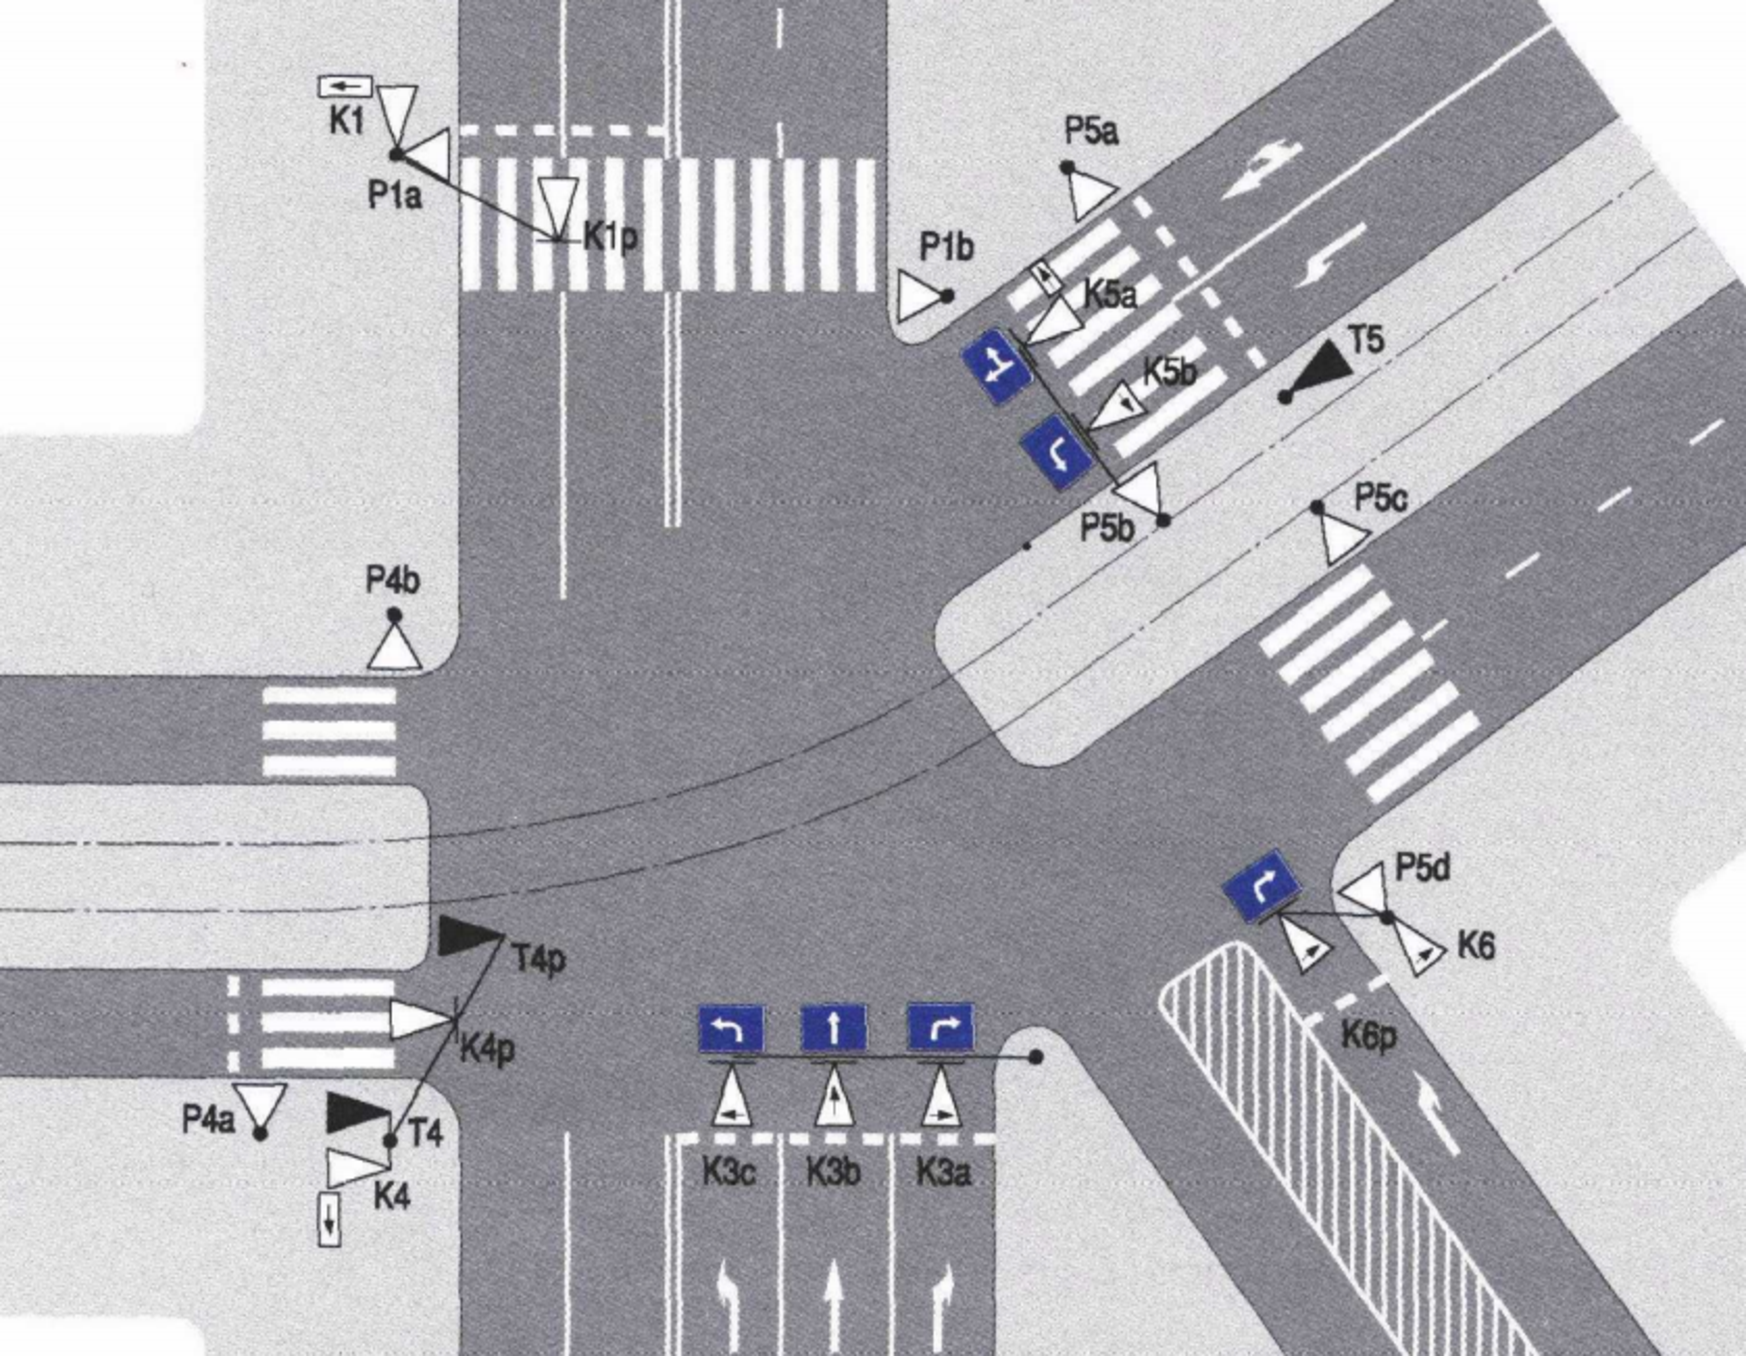
\includegraphics[scale=0.3]{schemat_1.pdf}\\
 {\tiny \textit{źródło: Rozporządzenie ministra infrastruktury z dnia 3 lipca 2003 r.}}
\end{frame}

\begin{frame}
 \frametitle{\vspace{22px}Sterowanie ruchem drogowym}
 Przepisy specyfikują wymagania dotyczące sterowania ruchem takie jak:
 \begin{itemize}
  \item{Wymagania czasowe trwania sygnałów}
  \item{Wymagania zapewniające bezpieczeństwo ruchu}
 \end{itemize}
 {\tiny Rozporządzenie ministra infrastruktury z dnia 3 lipca 2003 r. w sprawie szczegółowych warunków technicznych
 dla znaków i sygnałów drogowych oraz urządzeń bezpieczeństwa ruchu drogowego i warunków ich umieszczania na drogach.}
\end{frame}

\begin{frame}[shrink=5]
 \frametitle{\vspace{22px}Aktualne rozwiązania}
 \begin{itemize}
  \item{ITS - Wrocław - obszarowe sterowania ruchem, priorytet komunikacji zbiorowej}
  \item{Tristar - Trójmiasto - podobne do ITS, skupione na komunikacji zbiorowej}
 \end{itemize}
\end{frame}

\begin{frame}[shrink=5]
 \frametitle{\vspace{22px}Cel pracy}
 Opracowanie systemu sterowania ruchem drogowym na obszarze wzorowanym na okolicach placu Grunwaldzkiego we Wrocławiu.\\
 Porównanie opracowanego algorytmu sterowania ruchem z prostymi systemami sterowania.
\end{frame}

\begin{frame}[shrink=5]
 \frametitle{\vspace{22px}Cel pracy}
 \begin{itemize}
  \item{Badanie zachowania w zależności od natężenia na zadanych kierunkach}
  \item{Badanie zachowania dla nagłych zmian w ruchu}
 \end{itemize}
\end{frame}

\begin{frame}[shrink=5]
 \frametitle{\vspace{22px}Motywacja}
 Próba stworzenia systemu który nie trzyma się sztywnych ram programu sygnalizacji, jedynie stosuje się do zadanych ograniczeń.
\end{frame}

\begin{frame}[shrink=5]
 \frametitle{\vspace{22px}Opis systemu}
 \begin{itemize}
  \item{System rozproszony - obszar sterowania podzielony na podobszary (skrzyżowania) z własnymi sterownikami}
  \item{Sterowniki komunikują się ze sobą informując o przewidywanym ruchu}
  \item{Ciągła adaptacja do warunków ruchu}
  \item{Użycie algorytmów związanych z teorią sterowania}
 \end{itemize}
\end{frame}

\begin{frame}[shrink=5]
 \frametitle{\vspace{22px}Opis systemu}
 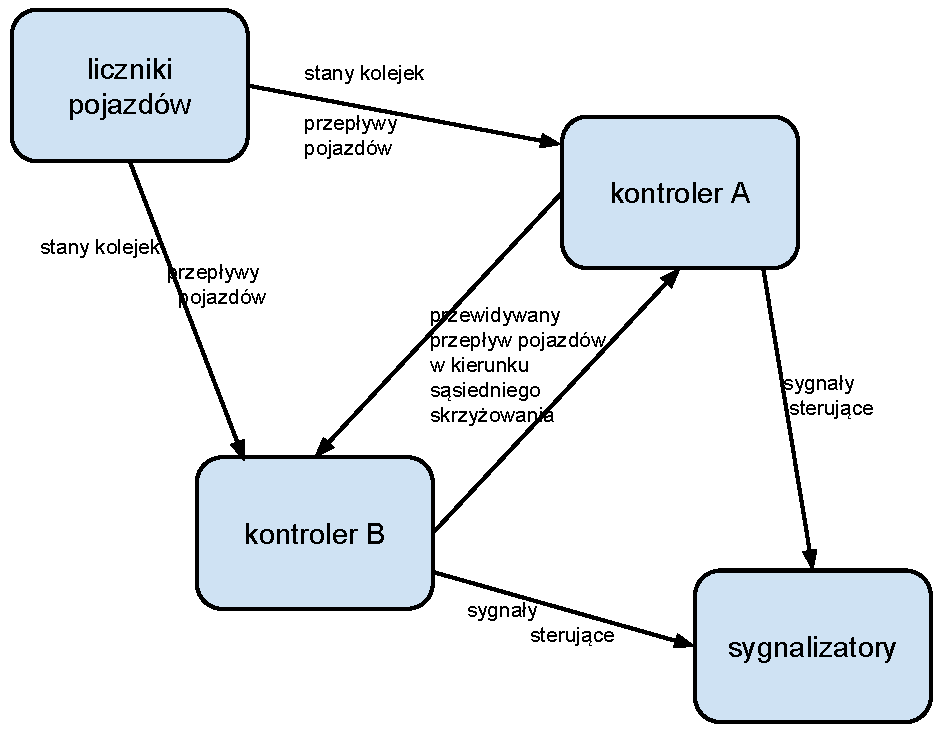
\includegraphics[scale=2]{schemat_0.pdf}
\end{frame}

\begin{frame}[shrink=5]
 \frametitle{\vspace{22px}Skrót Bibliografii}
 {\small
 \begin{itemize}
  \item{Kawalec, Piotr; Sobieszuk-Durka, Sylwia: Metody i algorytmy obszarowego sterowania ruchem drogowym. Prace Naukowe Politechniki Warszawskiej, Warszawa 2011}
  \item{Krawiec, Stanisław; Celiński, Ireneusz: Symulacja mikroskopowa ruchu w modelu obszarowym sieci drogowej. Prace Naukowe Politechniki Warszawskiej, Warszawa 2012}
 \end{itemize}
 }
\end{frame}

\begin{frame}[shrink=5]
 \frametitle{\vspace{22px}Skrót Bibliografii}
 {\small
 \begin{itemize}
  \item{Płaczek, Bartłomiej: Zastosowanie rozmytych automatów komórkowych do modelowania ruchu drogowego. Prace Naukowe Politechniki Warszawskiej, Warszawa 2012}
  \item{Rozporządzenie ministra infrastruktury z dnia 3 lipca 2003 r. w sprawie szczegółowych warunków technicznych
 dla znaków i sygnałów drogowych oraz urządzeń bezpieczeństwa ruchu drogowego i warunków ich umieszczania na drogach.}
 \end{itemize}
 }
\end{frame}

\end{document}
